\documentclass[12pt]{article}

\usepackage{graphicx}
\usepackage{url}
\usepackage{amsmath}
\usepackage[cm]{fullpage}
\usepackage{calc}
\usepackage{subfig}
\usepackage{float}

\title{\textbf{Wireless and Mobile Computing, Assignment 6}}
\author{Marcel Mohler \& Thomas Richner}
\begin{document}
\maketitle

\section{Setup}

We use a scenario where one station is a receiver and two stations send traffic to this receiver. Both sending stations make use of two ACs, hence send two data flows to the receiving station. The receiver therefore has four incoming flows.
We put all stations at the coordinates (0,0).

\begin{figure}[h!]
\centering
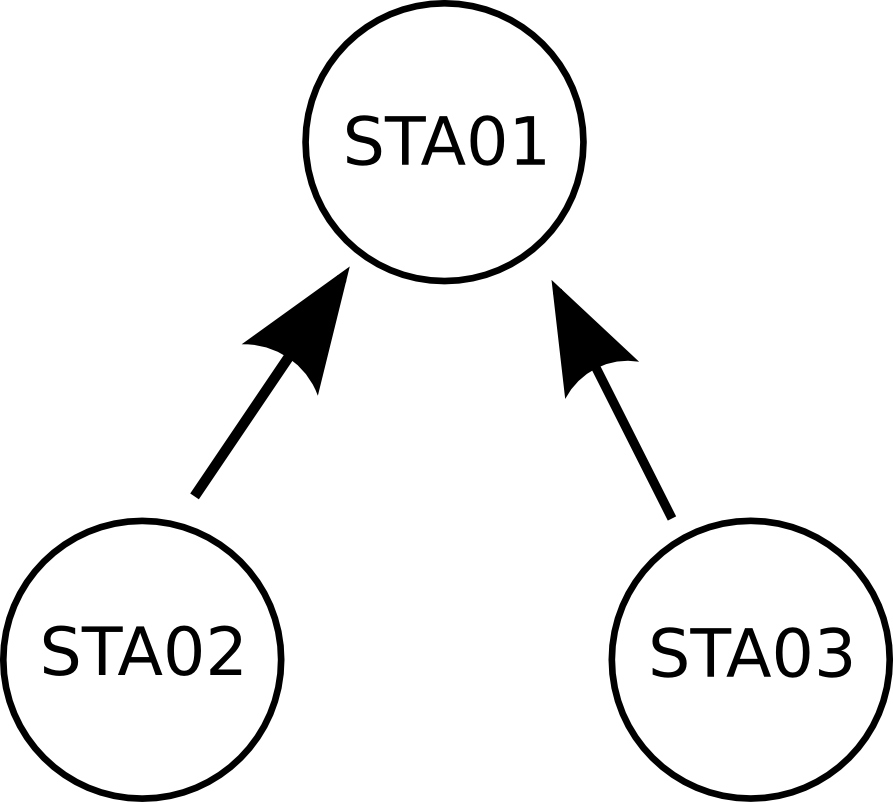
\includegraphics[width=80mm]{img/setup.png}
\caption{setup, receiver station and two sending stations \label{fig:setup}}
\end{figure}


\section{Algorithm Design "Anna"}

\subsection{Design Goals}
Our goal is to maximize the throughput per station under the following two constraints in order of their priority:
\begin{enumerate}
  \item Complete fairness against stations using the same algorithm which also results in no starvation. In case of two stations, both should achieve 50\% of the maximal throughput.
  We do not care about stations not using our algorithm at all.
  \item Basic 802.11e QoS support. We always prioritize AC1 over AC2. But if AC1 does not use the channel completely, AC2 should be allowed to fill it up.
\end{enumerate}

\subsection{Implementation}
We start by detecting how many other stations are using the same algorithm (TODO).
If we experience any other station using our algorithm as well we continue with Time Division Multiple Access (TDMA). Otherwise we behave totally selfish which means sending all the time without caring about others.
In theory the TDMA approach should prevent almost all collisions.
We do neither touch phymode nor power and leave these to their respective default values.

\subsection{Pseudo-Code}

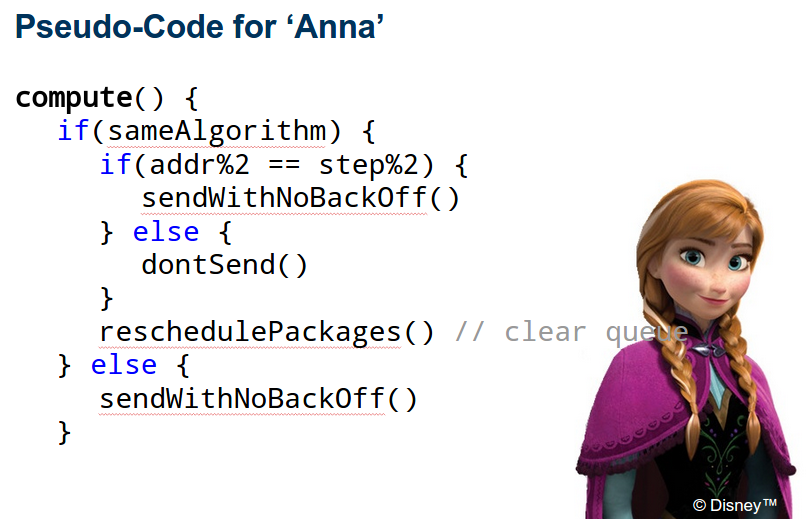
\includegraphics[width=160mm]{img/pseudocode.png}


\section{Evaluation}

\subsection{Measurements}

\subsection{Discussion \& Conclusion}


\section{Feedback}

\begin{description}
  \item[Difficulty] \hfill \\ appropriate
  \item[Clarity] \hfill \\ okay
  \item[Time Spent] \hfill \\ 10h
  \item[Conclusion] \hfill \\ 
\end{description}

\end{document}
